%Springer Nature LaTeX template, version 3.1 (December 2024)
\documentclass[pdflatex,sn-mathphys-num]{sn-jnl}

\usepackage{graphicx}%
\usepackage{multirow}%
\usepackage{amsmath,amssymb,amsfonts}%
\usepackage{xcolor}%
\usepackage{textcomp}%
\usepackage{booktabs}%
\usepackage{tabularx}%
\usepackage[T1]{fontenc}%
\usepackage[utf8]{inputenc}%

\newcommand{\todo}[1]{\textcolor{red}{[TO BE COMPLETED: #1]}}

\raggedbottom

\begin{document}

\title[Detecting Sexist Tweets (CLEF EXIST 2024)]{Project 3 -- Tweet Classification (CLEF EXIST Challenge): Detecting Sexist Tweets in English and Spanish}

\author{\fnm{Thibault} \sur{Gallapont}}
\author{\fnm{Arnaud} \sur{Malle}}
\author{\fnm{Thomas} \sur{Muel}}

\affil{\orgdiv{Natural Language Processing course, 5th year}, \orgname{INSA Lyon}, \orgaddress{\city{Lyon}, \country{France}}}

\abstract{We address Task~1 of the CLEF EXIST 2024 challenge: deciding whether a tweet, written in English or Spanish, is sexist. The task is subjective: each tweet was labelled by six annotators, only 32\% of the training tweets are unanimous, and tweets that report or denounce sexism also count as sexist. We compare TF-IDF models with a fine-tuned multilingual transformer pre-trained on tweets (Twitter-XLM-RoBERTa), trained on majority-vote (hard) labels and on the share of annotators who answered YES (soft labels). On the development set, TF-IDF reaches an F1 score of 0.781 on the YES class, the transformer 0.843, and the average of its hard- and soft-label versions 0.846, our best result. A second strategy inspired by the best teams (Spanish translated into English, large English models, handcrafted features, AEDA augmentation) stays between 0.833 and 0.848, within the $\pm$2.5-point uncertainty of our evaluation, for about three times the computing cost. Within our constraints, the simple multilingual model is the best trade-off.}

\keywords{sexism detection, social media, EXIST 2024, learning with disagreement, soft labels, multilingual transformers, data augmentation}

\maketitle

%=====================================================================================
\section{Introduction}\label{sec:intro}

Sexist content on social networks harms the people it targets and limits their freedom of expression online. Its volume makes manual moderation impossible, which motivates automatic detection. The EXIST campaign (\emph{sEXism Identification in Social neTworks}) has proposed shared tasks on this problem since 2021, in English and Spanish~\cite{plaza2024exist}. This project tackles Task~1 of EXIST 2024: deciding whether a tweet is sexist (YES) or not (NO).

\paragraph{Challenges.} Three properties make the task harder than an ordinary binary classification.
\begin{itemize}
\item \textbf{Subjectivity.} Each tweet was labelled by six annotators, three women and three men from three age groups, and they rarely agree: only 32\% of the training tweets receive a unanimous answer. EXIST follows the \emph{learning with disagreement} paradigm and provides all six answers instead of a single gold label~\cite{plaza2024exist}.
\item \textbf{A broad definition of sexism.} A tweet that \emph{reports} a sexist situation or \emph{denounces} sexism also counts as YES. Annotators who answer YES specify the intention of the tweet: DIRECT (sexist in itself), REPORTED or JUDGEMENTAL. About 55\% of YES votes are REPORTED or JUDGEMENTAL, so a sexist tweet and a tweet that criticises sexism often use the same words (``Women can't drive'' versus ``I'm sick of people saying women can't drive'').
\item \textbf{Bilingual, noisy text.} Tweets are short, informal, full of mentions, hashtags, emojis and slang, and split between English and Spanish.
\end{itemize}

\paragraph{Data.} We use the tweet part of the EXIST 2024 dataset, which is identical to the EXIST 2023 tweets: 6,920 training tweets and 1,038 development tweets. The labels of the official test set are not public, so the development set (``dev'') serves as our test set. The evaluation metric is the F1 score of the YES class, the F1 measure reported by EXIST for Task~1.

\paragraph{Contributions.} We (i)~analyse the dataset, in particular the disagreement between annotators; (ii)~build a reproducible pipeline that compares TF-IDF models with a multilingual transformer trained on hard or soft labels; (iii)~test a second strategy based on translation and large English models, with several additions taken from the literature; and (iv)~discuss which differences are actually measurable on a single development set.

%=====================================================================================
\section{State of the art}\label{sec:sota}

\subsection{The EXIST challenge and learning with disagreement}

The EXIST 2024 overview~\cite{plaza2024exist} describes the six tasks of the campaign (identification, source intention and categorisation, for tweets and memes), the dataset and the systems of 57 teams. It defines two evaluation settings: a \emph{hard} setting, where the gold label is obtained by majority vote, and a \emph{soft} setting, where the gold label is the distribution of the annotators' answers. Nearly all participants used pre-trained transformers (BERT, RoBERTa, XLM-RoBERTa, DeBERTa); some added large language models (LLMs) used in zero- or few-shot mode. EXIST 2025~\cite{plaza2025exist} reuses exactly the same tweets, so its results are directly comparable.

Table~\ref{tab:top} summarises the best systems. All of them rely on \emph{large} models or on generative LLMs.

\begin{table}[h]
\caption{Best systems on Task~1 (hard setting) of EXIST, F1 of the YES class on the official \emph{test} set~\cite{plaza2024exist,plaza2025exist}.}\label{tab:top}
\begin{tabularx}{\textwidth}{@{}llcX@{}}
\toprule
Rank & Team & F1 & Main ingredients \\
\midrule
1st, 2024 & NYCU-NLP~\cite{fang2024nycu} & 0.794 & DeBERTa-v3-large and XLM-R-large, back-translation, AEDA, annotator information, multi-task learning, 5-fold cross-validation \\
2nd, 2024 & ABCD Team & 0.783 & one model per annotator group, then aggregation \\
3rd, 2024 & CIMAT-CS-NLP & 0.790 & ensemble of a zero-shot LLM (Gemini) and fine-tuned XLM-R \\
4th, 2024 & EquityExplorers & 0.778 & Spanish translated into English, fusion of RoBERTa-large and DeBERTa-v3-large \\
1st, 2025 & Mario~\cite{mario2025} & 0.817 & Llama-3.1-8B fine-tuned with QLoRA \\
2nd, 2025 & CIMAT-GTO~\cite{cimat2025knowledge} & 0.800 & LLM-generated justifications added to the tweet before Twitter-XLM-R \\
\botrule
\end{tabularx}
\end{table}

\subsection{Models and resources}

\paragraph{Pre-trained models.} Twitter-XLM-RoBERTa~\cite{barbieri2022xlmt} is a multilingual model further trained on about 200 million tweets. BERTweet~\cite{nguyen2020bertweet} is trained on 850 million English tweets; its large version performs best on the EDOS sexism dataset~\cite{alazzawi2023nlpltu,kirk2023edos}, on which fine-tuned models are publicly available~\cite{nlpltu_model,rydelek2023adamr}.

\paragraph{Augmentation and architectures.} AEDA~\cite{karimi2021aeda}, which only inserts random punctuation, outperforms EDA~\cite{wei2019eda}, which changes words. A convolutional head on top of BERT (MultiCNN) slightly improves sexism detection~\cite{kalra2021sexism}, and several teams predict more than two classes~\cite{chen2025beyond,fang2024nycu,nowakowski2025grootwatch}. For translation, we used MarianMT~\cite{marianmt} and NLLB-200~\cite{nllb2022}.

\paragraph{Libraries.} Our pipelines are built with scikit-learn for the TF-IDF models, and with PyTorch and Hugging Face Transformers~\cite{wolf2020transformers} for the transformers.

\subsection{Limits of the existing approaches for our setting}

The literature leaves several gaps for a student project with our constraints.
\begin{itemize}
\item \textbf{The largest gains come from generative LLMs}: LLM-generated justifications raise the validation F1 of CIMAT-GTO from 0.829 to 0.859~\cite{cimat2024stacked}, and the 2025 winner fine-tunes an 8-billion-parameter LLM~\cite{mario2025}. Sending uncertain tweets to an LLM adds 1 to 1.5 points~\cite{alajmi2025warwick}. These approaches need large GPUs or paid APIs, and we chose to stay within the BERT family.
\item \textbf{Only the development set is available.} The labels of the official test set are not public, so all our results are measured on the dev set and cannot be placed directly in the official rankings.
\item \textbf{Sexism-specific models use another definition.} EDOS defines sexism as ``any abuse, implicit or explicit, that is directed towards women based on their gender''~\cite{kirk2023edos}; EXIST also includes tweets that report or denounce sexism. An EDOS model cannot be used without retraining.
\item \textbf{Results on the development set are optimistic.} Every team loses several points between its validation and the test set (CIMAT-GTO drops from 0.859 to 0.789), and feature selection tuned on the development data may not generalise~\cite{chaviaras2026ails}.
\end{itemize}

%=====================================================================================
\section{Contribution}\label{sec:contrib}

\subsection{Approach}

Our approach has two stages. The \emph{main pipeline} starts from simple TF-IDF models to obtain a reference, then fine-tunes one multilingual transformer that handles both languages directly, trained on hard labels, on soft labels, and finally averaged. The \emph{second pipeline} reproduces the ideas of the best teams that remain within our constraints: translate everything into English to use stronger English models, start from a model already specialised in sexism, and add features, augmentation and alternative heads. All experiments use the same split and the same metric, so that the two pipelines can be compared.

\subsection{Dataset and statistics}

The dataset is distributed as JSON files with, for each tweet, its text, its language, the six answers to each task and a profile of each annotator. From the six answers to Task~1 we derive two labels: the \textbf{hard} label (YES if at least 4 annotators out of 6 answered YES, NO if at most 2; 3--3 ties are discarded, as in the official hard evaluation) and the \textbf{soft} label $p$, the share of YES answers (e.g.\ $4/6 \approx 0.67$). Table~\ref{tab:data} and Figure~\ref{fig:data} summarise the data.

\begin{table}[h]
\caption{Dataset statistics (hard labels).}\label{tab:data}
\begin{tabular}{@{}lcc@{}}
\toprule
 & Train & Dev \\
\midrule
Tweets & 6,920 (3,260 EN, 3,660 ES) & 1,038 (489 EN, 549 ES) \\
YES & 2,697 (39\%) & 455 (44\%) \\
NO & 3,367 (49\%) & 479 (46\%) \\
3--3 ties (discarded) & 856 (12\%) & 104 (10\%) \\
Share of YES, English / Spanish & 40\% / 49\% & 44\% / 53\% \\
\botrule
\end{tabular}
\end{table}

\begin{figure}[h]
\centering
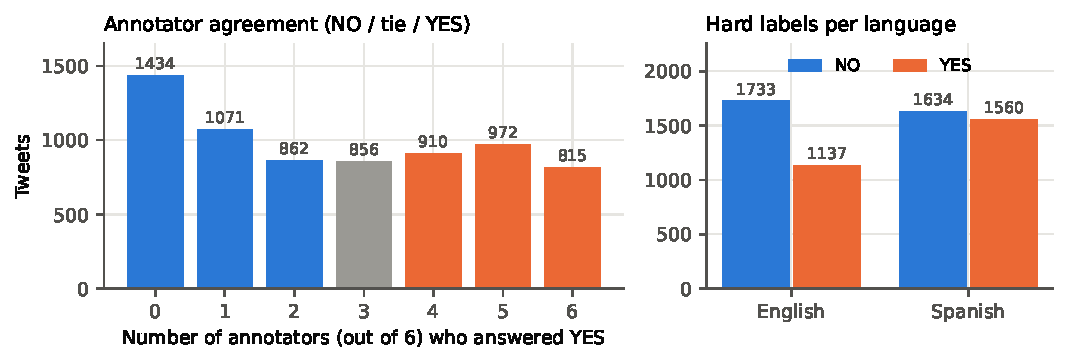
\includegraphics[width=\textwidth]{figures/fig_data.pdf}
\caption{Training set. Left: number of annotators who answered YES; unanimity (0 or 6) concerns only 32\% of the tweets. Right: hard labels per language.}\label{fig:data}
\end{figure}

The exploratory analysis revealed several properties that guided our choices.
\begin{itemize}
\item \textbf{Annotator severity varies enormously.} Depending on the annotator, the share of YES answers ranges from 0.07 to 0.93, and from 0.21 to 0.63 depending on the group of six. Part of each label therefore depends on which group annotated the tweet, which is noise for a model.
\item \textbf{Some surface signals are informative} (Table~\ref{tab:signals}). URLs and hashtags point to non-sexist tweets, because many come from awareness campaigns (8\% of YES for \#WomensDay); some emojis are telling (73\% of YES for the eye-roll emoji, 17\% for a heart).
\item \textbf{Collection keywords bias the models}: tweets containing \emph{women} or \emph{mujeres} are YES in 77\% and 85\% of cases, which pushes a model to equate ``talking about women'' with ``sexist''.
\item \textbf{Tweets are short} (177 characters on average, only 0.2\% exceed 160 tokens), and the data contain a few near-duplicates with contradictory labels and eight tweets that only contain an automatic message. The train and dev sets share practically no tweet.
\end{itemize}

\begin{table}[h]
\caption{Surface signals in the training tweets with a hard label.}\label{tab:signals}
\begin{tabular}{@{}lccc@{}}
\toprule
Element & Share of tweets & YES when present & YES otherwise \\
\midrule
URL & 31\% & 36\% & 49\% \\
Hashtag & 14\% & 32\% & 47\% \\
Reply (starts with a mention) & 47\% & 49\% & 41\% \\
Emoji & 18\% & 41\% & 45\% \\
Laughter (``jaja'', ``lol'') & 2\% & 60\% & 44\% \\
\botrule
\end{tabular}
\end{table}

\subsection{Workflow}

\paragraph{Preprocessing.} Cleaning is deliberately light: HTML entities are decoded, URLs become \emph{url}, mentions become \emph{@user} (so that the model does not learn account names), hashtags are kept and split on capital letters (\#IDoNotRenounce becomes ``i do not renounce''), and repeated letters are shortened. Stopwords are kept: two lists would be needed, and words such as \emph{not} or \emph{she} matter here. We keep a lowercase version for TF-IDF and a cased version for the transformers, which were pre-trained on raw text.

\paragraph{Indicator words.} We built, from the training set only, a short list of words whose use almost always signals a sexist tweet: 16 English words (e.g.\ \emph{whore}, \emph{feminazi}, \emph{dumb blonde}) and 13 Spanish words (e.g.\ \emph{zorra}, \emph{marimacho}, \emph{sumisa}), each YES in at least 80\% of its occurrences. General insults such as \emph{bitch} or \emph{puta} were excluded because they also appear in many non-sexist tweets. When a tweet contains one of these words, a marker token is appended so that TF-IDF learns a single, more reliable weight for these rare words. The list is reliable (93--95\% of the marked tweets are sexist) but covers only 12--18\% of the sexist tweets.

\paragraph{TF-IDF models.} Tweets are represented by TF-IDF vectors over word unigrams and bigrams, optionally concatenated with character 2- to 5-grams, which are robust to misspellings, slang and variants. We compare a majority-class baseline, three linear models (logistic regression, linear SVM, ridge classifier), Complement Naive Bayes, and two tree-based models (random forest, XGBoost), with balanced class weights where possible.

\paragraph{Soft labels.} scikit-learn does not accept targets between 0 and 1, so each tweet is duplicated: once labelled YES with weight $p$ and once labelled NO with weight $1-p$. The logistic regression then minimises exactly the cross-entropy between its prediction $\hat p$ and the annotators' distribution, $-\left[p \log \hat p + (1-p)\log(1-\hat p)\right]$. Soft labels also let us use the 856 tied tweets.

\paragraph{Transformer.} We fine-tune Twitter-XLM-RoBERTa base~\cite{barbieri2022xlmt}: it is multilingual, so a single model handles both languages without translation, and it already knows the style of tweets. A two-class layer is added on top of the encoder. We wrote our own PyTorch training loop so that the same cross-entropy can be used with hard targets ($p \in \{0,1\}$) or soft targets. Settings: 3 epochs, AdamW (learning rate $2\cdot10^{-5}$, weight decay 0.01), linear schedule with 10\% warm-up, batch size 16, at most 128 tokens, half precision on an RTX 3070 laptop GPU. We keep the epoch with the lowest validation cross-entropy. The final model averages the probabilities of the hard- and soft-label versions, which requires no extra training.

\paragraph{Second pipeline.} This pipeline ran on Google Colab with a larger GPU.
\begin{itemize}
\item \textbf{Translation.} Spanish tweets are translated into English with NLLB-200 (3.3B parameters)~\cite{nllb2022}; the dev set is translated at prediction time, which is not a leak since the model never trains on it. Emojis are removed before translation and added back afterwards, and the \emph{@USER}/\emph{HTTPURL} tokens are repaired when the translation alters them.
\item \textbf{Models.} BERTweet-large~\cite{nguyen2020bertweet}, either generic or already fine-tuned on EDOS~\cite{nlpltu_model}. Because of the definition gap with EDOS, the EDOS model is retrained on EXIST.
\item \textbf{Additions.} 21 handcrafted features computed on the original tweet (indicator words, generalisations such as ``women are\dots'', gendered insults, campaign hashtags, emojis, etc.), added to the output scores through a zero-initialised linear layer; AEDA augmentation~\cite{karimi2021aeda}; a MultiCNN head~\cite{kalra2021sexism}; and a four-class output (NO, DIRECT, REPORTED, JUDGEMENTAL) trained on the distribution of the six votes, with $P(\text{YES}) = 1 - P(\text{NO})$.
\end{itemize}
In the main pipeline, we also tested data augmentation by translation: every English tweet is translated into Spanish and every Spanish tweet into English with MarianMT~\cite{marianmt}, keeping the annotations, which doubles the training set (13,840 tweets). It is disabled by default in our notebook because it roughly triples the running time.

\subsection{Evaluation methods}

\begin{itemize}
\item \textbf{Split.} Models are trained on the training set and evaluated on the dev set, never used for training. 10\% of the training set (always the same draw, seed 42) is held out as a validation set to choose the epoch of the transformers.
\item \textbf{Main metric.} The F1 score of the YES class, $F_1 = 2PR/(P+R)$ where $P$ and $R$ are the precision and recall of YES, computed on the 934 dev tweets that have a hard label. We also report the accuracy and the macro-F1.
\item \textbf{Soft metric.} The cross-entropy between predicted probabilities and the share of YES answers on the whole dev set, which measures how well a model reproduces the annotators' disagreement (lower is better). It is close in spirit to the soft evaluation of EXIST, which uses the ICM-soft measure.
\item \textbf{Uncertainty.} With 934 tweets, the 95\% confidence interval of an F1 score is about $\pm$2.5 points. We use it to decide which differences are meaningful.
\end{itemize}

\subsection{Experiments and results}

\paragraph{TF-IDF models.} Figure~\ref{fig:tfidf} and Table~\ref{tab:tfidf} show that the three linear models clearly lead, at about 0.78 with character n-grams, which add 1 to 2.5 points. Naive Bayes and the tree-based models stay behind: on high-dimensional sparse vectors, non-linearity brings nothing and costs much computing time. The indicator words do not help (0.778 versus 0.781): TF-IDF already sees each of these words, and they concern few tweets. Note that the best TF-IDF model was chosen on the dev set, so its score is slightly optimistic.

\begin{figure}[h]
\centering
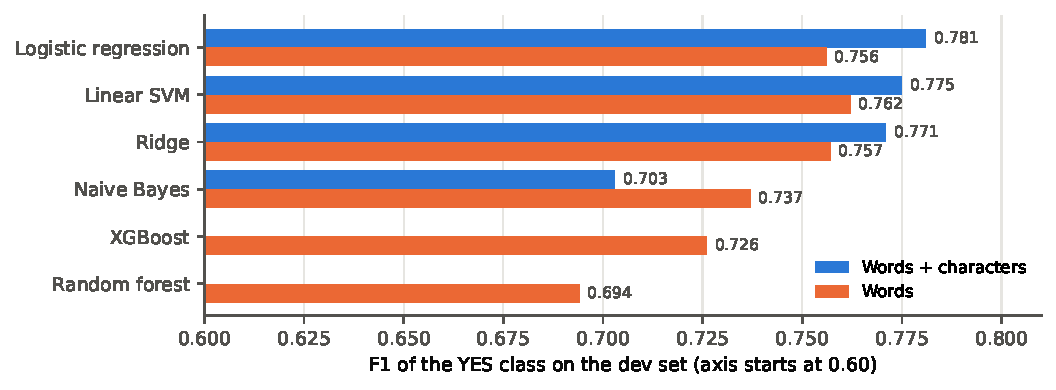
\includegraphics[width=\textwidth]{figures/fig_tfidf.pdf}
\caption{TF-IDF models: F1 of the YES class on the dev set. Tree-based models were only trained on word features because of their cost.}\label{fig:tfidf}
\end{figure}

\begin{table}[h]
\caption{Best TF-IDF models on the dev set. The majority-class baseline has an F1 of 0 (it never predicts YES) and a macro-F1 of 0.339.}\label{tab:tfidf}
\begin{tabular}{@{}llccc@{}}
\toprule
Features & Model & Accuracy & F1 (YES) & Macro-F1 \\
\midrule
Words + characters & Logistic regression & 0.792 & \textbf{0.781} & 0.792 \\
Words + characters & Linear SVM & 0.786 & 0.775 & 0.785 \\
Words + characters & Ridge & 0.784 & 0.771 & 0.783 \\
Words + characters + indicator words & Logistic regression & 0.791 & 0.778 & 0.790 \\
Words & Linear SVM & 0.775 & 0.762 & 0.774 \\
\botrule
\end{tabular}
\end{table}

\paragraph{Error analysis.} Errors concentrate on ambiguous tweets (Figure~\ref{fig:errors}): the logistic regression is wrong on 11--15\% of the unanimous tweets but on 39\% of the tweets that received 4 YES out of 6. Its most influential YES features are \emph{women}, \emph{mujeres}, \emph{mujer}, \emph{feminazi}, \emph{feminismo} and insults: the model reacts to words rather than meaning, whereas a tweet that denounces sexism uses the same words as a sexist one.

\begin{figure}[h]
\centering
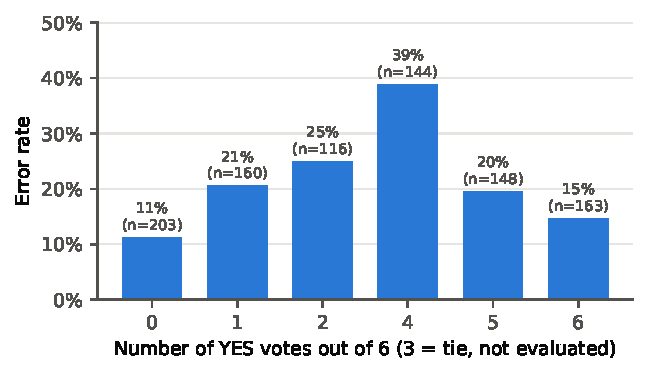
\includegraphics[width=0.65\textwidth]{figures/fig_errors.pdf}
\caption{Error rate of the TF-IDF logistic regression on the dev set, by number of YES votes.}\label{fig:errors}
\end{figure}

\paragraph{Soft labels with TF-IDF.} Training on soft labels barely changes the F1 (0.775 versus 0.781) but lowers the cross-entropy from 0.614 to 0.571: the model is less categorical on ambiguous tweets.

\paragraph{Transformer.} Table~\ref{tab:roberta} shows that fine-tuning the transformer brings the only clear gain of the project, +6.5 points over TF-IDF, in both languages (0.833 in English and 0.850 in Spanish for the hard version). With hard labels, the validation cross-entropy rises from the second epoch while the training loss keeps decreasing (Figure~\ref{fig:curves}): the model becomes over-confident, which is why we keep the best epoch. With soft labels, the curve stays flat, since the model cannot be more categorical than the annotators. The hard version has the best F1, the soft version the most faithful probabilities (cross-entropy 0.533 versus 0.658), and their average combines both: the best F1 of the main pipeline (0.846) with a cross-entropy of 0.541. The gain of the average stays small because both versions start from the same model and see the same tweets.

\begin{table}[h]
\caption{Main pipeline on the dev set.}\label{tab:roberta}
\begin{tabular}{@{}lcc@{}}
\toprule
Model & F1 (YES) & Cross-entropy \\
\midrule
TF-IDF, hard labels & 0.781 & 0.614 \\
TF-IDF, soft labels & 0.775 & 0.571 \\
Twitter-XLM-R, hard labels & 0.843 & 0.658 \\
Twitter-XLM-R, soft labels & 0.834 & \textbf{0.533} \\
\textbf{Twitter-XLM-R, average of hard and soft} & \textbf{0.846} & 0.541 \\
\botrule
\end{tabular}
\end{table}

\begin{figure}[h]
\centering
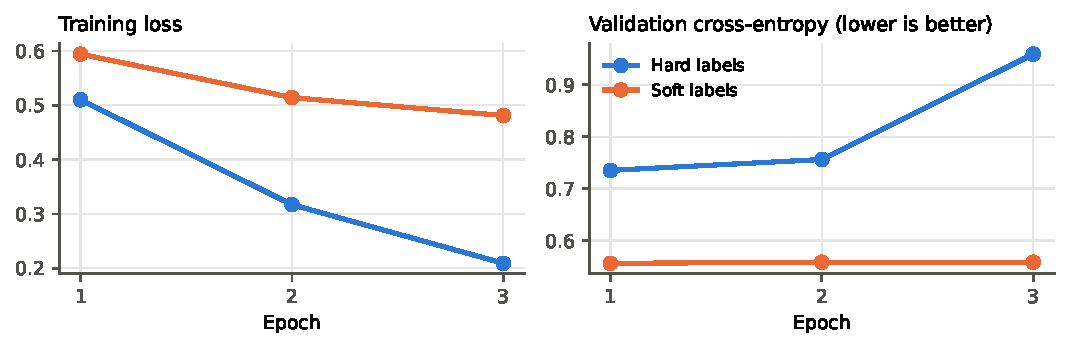
\includegraphics[width=\textwidth]{figures/fig_roberta_curves.pdf}
\caption{Fine-tuning of Twitter-XLM-RoBERTa. The hard-label model over-fits after the first epoch; the soft-label model stays stable.}\label{fig:curves}
\end{figure}

\paragraph{Translation as data augmentation.} Doubling the training set with MarianMT translations brought nothing: no gain for TF-IDF, $-1.4$ points for the hard transformer and $+0.4$ for the soft one. Since the model is already multilingual, a translated copy teaches it little, adds translation errors (some tweets labelled Spanish are actually Galician), and speeds up over-fitting, because each tweet is seen twice per epoch.

\paragraph{Second pipeline.} All configurations of the translation + BERTweet strategy score between 0.833 and 0.848 (Table~\ref{tab:second}), and their ranking changes between validation and dev, so these differences are noise. Neither the MultiCNN head, the features nor longer training brings a measurable gain, and starting from the EDOS model helps at most slightly. Translation also adds errors (``bancarrota'' becomes ``BANK ROTA''): translated Spanish scores below English, whereas untranslated Spanish scored above English in the main pipeline.

\begin{table}[h]
\caption{Second pipeline (Spanish translated into English, BERTweet-large models). ``EDOS detector'' is the BERTweet-large model already fine-tuned on EDOS, retrained on EXIST.}\label{tab:second}
\begin{tabular}{@{}lcc@{}}
\toprule
Model & F1 validation & F1 dev \\
\midrule
BERTweet-large + linear head & 0.845 & 0.833 \\
BERTweet-large + MultiCNN + features & 0.843 & 0.846 \\
EDOS detector + linear head & 0.845 & 0.847 \\
EDOS detector + MultiCNN + features & 0.838 & 0.848 \\
EDOS detector + linear + features, early stopping & 0.836 & 0.848 \\
EDOS detector + linear + features, 4 epochs & 0.844 & 0.839 \\
\botrule
\end{tabular}
\end{table}

\paragraph{Summary.} Figure~\ref{fig:summary} gathers all configurations. With 934 dev tweets, the 95\% uncertainty of an F1 score is about $\pm$2.5 points: apart from the jump from TF-IDF to transformers, every difference between our models is within this margin. The large English models cost about three times more computation per tweet, plus the cost of translation, for no measurable gain. For reference, the best F1 scores on the official \emph{test} set were 0.794 in 2024 and 0.817 in 2025; our scores are measured on the dev set and are therefore not directly comparable.

\begin{figure}[h]
\centering
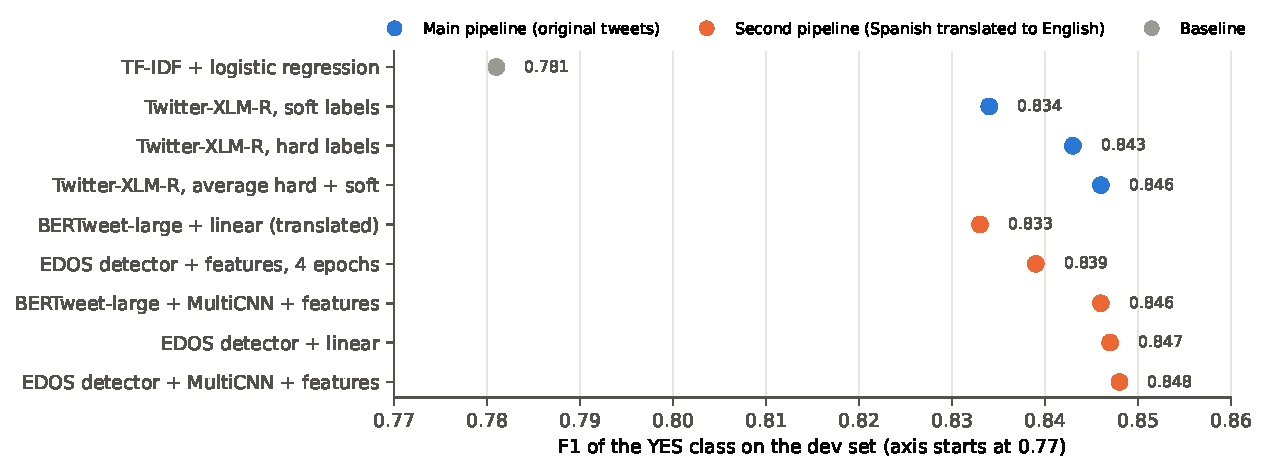
\includegraphics[width=\textwidth]{figures/fig_summary.pdf}
\caption{F1 of the YES class on the dev set for all configurations.}\label{fig:summary}
\end{figure}

%=====================================================================================
\section{Conclusion}\label{sec:conclusion}

Fine-tuning a multilingual transformer pre-trained on tweets is the decisive step for detecting sexist tweets in English and Spanish: it raises the F1 of the YES class from 0.781 with TF-IDF to 0.843, and to 0.846 when the hard- and soft-label versions are averaged. Soft labels change the F1 little, but they give probabilities that follow the annotators' disagreement and they limit over-fitting. Translation, large English models, an EDOS-specialised model, handcrafted features, AEDA, a convolutional head and a four-class output did not bring any measurable improvement. We therefore retain the simplest and cheapest model, which handles both languages without translation.

\subsection{Contribution of each team member}

All three of us worked on every part of the project, and each of us also took charge of one part. Thibault wrote the initial notebook, with the TF-IDF models, the linear classifiers and the fine-tuning of the BERT model. Arnaud made the presentation and its figures, and helped with the BERT model. Thomas analysed the other EXIST teams, read the research papers and tested the BERT models of the second pipeline. For all of us, the most difficult part was finding the right BERT model: we had to launch many trainings, each of them very long, and most differences turned out to be within the uncertainty of our evaluation. The most interesting parts were the analysis of the data, in particular the disagreement between annotators, and the study of the state of the art and of the results of the other teams, to understand how they had built their systems.

\subsection{Limitations}

\begin{itemize}
\item \textbf{A single, small evaluation set.} With 934 dev tweets, the uncertainty of an F1 score ($\pm$2.5 points) is larger than all the differences between our best models, and the 684-tweet validation set is noisy too, which makes the choice of epochs and models imprecise.
\item \textbf{One seed per configuration.} Part of the differences comes from the randomness of training (initialisation, order of examples, AEDA draws), which also explains why rankings change between validation and dev.
\item \textbf{Imperfect comparisons.} In one experiment only the MultiCNN heads received the features, one run had a badly tuned learning-rate schedule, and the GPU and numerical precision differ between the two pipelines. The best TF-IDF model was selected on the dev set.
\item \textbf{The subjectivity of the task.} A large part of the remaining errors concerns tweets on which the annotators disagree, and part of each label depends on the severity of the group that annotated it; a model cannot fully resolve this noise.
\item \textbf{Constraints we imposed.} We excluded generative LLMs, which give the best published results, and we could not use annotator information.
\end{itemize}

\subsection{Perspectives}

\begin{itemize}
\item \textbf{Measure more reliably}: several seeds per model with averaged probabilities, and 5-fold cross-validation instead of a single 10\% validation set.
\item \textbf{Larger multilingual models} on the original tweets (XLM-RoBERTa-large, mDeBERTa-v3), as in the winning system of 2024~\cite{fang2024nycu}.
\item \textbf{Multi-task learning} that also predicts Tasks~2 and~3 (intention and type of sexism), which are already annotated in the dataset and could help the model separate sexist tweets from tweets that denounce sexism.
\item \textbf{Beyond our constraints}: LLM-generated justifications~\cite{cimat2024stacked}, fine-tuning an LLM~\cite{mario2025}, or routing uncertain tweets to an LLM~\cite{alajmi2025warwick}.
\end{itemize}

\backmatter

\bmhead{Code and data availability}
The notebook of the main pipeline (\emph{Modelling.ipynb}) and the EXIST 2024 tweets used in this work are stored in the private repository of the project.

\bibliography{references}

\end{document}
